\documentclass[12pt, notitlepage]{article}

\usepackage[letterpaper, margin=1in]{geometry}
\usepackage{graphicx}

\setlength\parindent{0pt}

\title{Interactive comment to ``The Aerosol Limb Imager: acousto-optic imaging of limb scattered
sunlight for stratospheric aerosol profiling'' by B. J. Elash et al}

\author{B.~J. Elash et al. (brenden.elash@usask.ca)}

\begin{document}

\begin{titlepage}
\maketitle
\end{titlepage}


We would like to thank Dr. Dekemper for his helpful comments and suggestions. Below are the referee's comments in italics followed by our reply. A full list of changes can be seen in the attached file.

\hrulefill

\textit{1) I am not sure that the introduction section should be so long. To me, regarding the
scope of the paper, the not-so-concise discussion on previous limb missions having
measured stratospheric aerosols is not helping in appreciating the work done here.
Shortening this part could free some space for some missing information in the calibration
section or for the error analysis.}\\

\textbf{Reply:} The discussion of previous aerosol missions is relevant in regard to the work presented here. The motivating work behind ALI is to eventually use an ALI type instrument on a microsat mission to continue the global aerosol record. Outlining this information in detail is fundamental to understanding the purpose behind the ALI instrument and its mission.

\hrulefill

\textit{2) p. 13290, l. 23-24: the width of the spectral transmission function of an AOTF
is something which is frozen at the manufacturing step, i.e. when the crystal cutting
angles are frozen. In that sense, there is no such thing like typical bandwidths, as one
can design an AOTF with a 5-10 times narrower or broader bandpass.}\\

\textbf{Reply:} Yes this is correct and the phrasing of this sentence does not adequately reflect this possibility of the AOTF design, as such the sentence has been reworded into the following: ``Additionally, the spectral bandpass of the AOTF has reasonable resolutions at these wavelengths, such as 3--6\,nm, which is very suitable for the broadband scattering characteristics of the aerosol limb signal.''

\hrulefill

\textit{3) p. 13291, l. 24: The acoustic wave in this kind of device is not a standing wave. In
TeO2 AOTF, it is a shear wave mostly absorbed at the opposite end of the crystal.}\\

\textbf{Reply:} Noted and has been corrected.

\hrulefill

\textit{4) AOTF design. There is an extensive discussion on the selection of the most appropriate
optical design which is well argued. However, I wonder why the rear facet of the
AOTF was cut such as depicted in fig.2 (by the way, replace "standing RF" by "acoustic"
in this figure). From the moment it is decided to work with the e-light as input, a
better configuration could have been found where the diffracted beam remains parallel
to the incident axis and a larger angular separation is achieved with the 0-order. This is
important because with a half-FOV of 3◦, and taking into account your drawing and the
fact that the diffracted beam leaves the crystal with an angle of 2.7◦, there should be a
significant overlapping of the 0th and 1st orders\ldots Could you better justify this design
choice in the text?}\\

\textbf{Reply:} The geometry in Fig. 2 is meant to be a representation of the diffraction interactions within the AOTF and not accurate to physical geometry. The text has been changed to: ``A representative AOTF\ldots'' and the phase ``standing RF'' and been replaced with ``acoustic''. Although the diffraction angle is 2.7$^{\circ}$ the separation between the zeroth and first order is at minimum 6.4$^{\circ}$ which alleviates any concern with 0th order and 1st order overlap. The addition of the separation angle has been added into the text in the following sentence ``\ldots in this way and is diffracted 2.7◦ from the input optical axis of the device with a minimum separation angle of 6.4$^{\circ}$ between the zeroth and first order.'' (pg 13293, line 18). The 2.7$^{\circ}$ offset was just a feature of the AOTF that we purchased from the selection available at the time.

\hrulefill

\textit{5) I think the section 2.2 should contain a proper mathematical description of the radiometric
model of the instrument, including the spectral transmission function, the
polarization sensitivity and other effects such as PRNU. This would certainly help in
understanting the impact of the calibration uncertainties when discussing the error budget.}\\

\textbf{Reply:} A complete radiometric model has not been necessary for this project; however additional detail is provided in the results section outlining where the primary error terms arise in the formation of the measurement vector and how this effect the final uncertainty estimation.

\hrulefill

\textit{6) p. 13299, l. 14-15: I would not say that 1.2nm is much less than the AOTF spectral
resolution. You indeed performed a characterization of the spectral transmission
function of the AOTF with a not-exactly monochromatic light source. In the end you got
a result (fig.6a) which is the convolution of the incident light spectrum and the AOTF
response. The typical sidelobes are not completely resolved, but this is not really an
issue for your calibration as the results seem perfectly in line with standard AOTF performance.
I would recommend next time to work with sharp emission lines or laser lines
at some selected wavelengths, and rely on the physics of acousto-optic interaction to
extrapolate the AOTF response function between the calibration points.}\\

\textbf{Reply:} This is a good suggestion in addition to our characterization and will be considered for future ALI development.

\hrulefill

\textit{7) Section 3.1: Why didn’t you use a physical model to fit the experimental data with
the AOTF tuning curve? This would provide a better understanding of the overall instrument.
Also, as the F(lambda) relationship is dependent on the crystal temperature,
it would be usefull to compare the temperature in the lab when the calibration of the
instrument was done with the temperature of the crystal during the flight. Again, a
physical model of the AOTF would help in extrapolating the calibration to other working
temperatures. The reported 0.1\% error in the fit can yield an uncertainty as high as
1nm. A 10◦C shift of temperature would also yield a 1nm drift. Is this still tolerable for
your measurements? More details on the precision of the wavelength selection would
be appreciated.}\\

\textbf{Reply:} Although a physical model could have been selected to model the AOTF, a fit was selected since a full wavelength calibration was performed. For the model used, a  maximum error of 1\,nm is possible from the wavelength calibration with the addition of another 1.5\,nm error from the temperature changes. The error in the temperature is estimated by considering the difference from the lab calibration temperatures to the flight temperatures to be approximately 15$^{\circ}$C. Overall, this amounts to a possible wavelength error of 2.5\,nm. With the slowly varying broadband scattering effects of aerosol this error in the wavelength is not a large concern for this prototype and  has small effect on the retrieval. The text has been modified in the following way to clarify these concerns with the addition of the following sentence ``\ldots(see Fig.~6b). Even with considering the temperature change, the AOTF would experience a maximum wavelength drift of 2.5\,nm during the the mission which is acceptable for the slowly varying broadband scattering cross section of aerosol.''.

\hrulefill

\textit{8) Section 3.2: It is mentioned that a diffraction efficiency of 54-64\% is observed, but
nothing is said concerning the power applied to the transducer of the crystal. Also,
these values appear quite low compared to typical DE for TeO2 easily reaching 90\%.
Moreover the method described neglects the attenuation by the crystal itself, and it is
not clear if the incident light was initially polarized. I would recommend to re-write this
section such that one can better understand how these values could be obtained.}\\

\textbf{Reply:} Our crystal was rated for 2\,W RF and the power pumped into the crystal was approximately 2.0\,W. As the RF power was increased, the DE increased. However we did not want to exceed the power rating for our crystal. The DE that was determined by our tests were close to the factory specified DE of 60\%. The light entering the system was linearly polarized, aligned with the AOTF's polarization axis. Lastly the attenuation of the signal from the AOTF is technically a loss of signal and not a change in the DE but was never calculated as the two effects were lumped together in our analysis and a note has been made about this in the text. See section 3.1 for the complete changes to this section.

\hrulefill

\textit{9) Stray light: Cycling between the ON/OFF state of the AOTF is probably a unique
feature of the AOTF which is well emphasized in the text. However, knowing how
complex straylight characterization can be, I wonder why all these efforts were made
as in the end, the problem is mostly solved by the ON/OFF approach. The only effect
which is not solved by the ON/OFF method is the straylight generated after the AOTF.
Is there something that can be said on this based on the characterization that was
performed?}\\

\textbf{Reply:} The propagation directions of the non-desired orders passing through the AOTF are slightly altered by the acoustic wave. As such work was done to verify that an ON/OFF approach would be able to remove most of the unwanted signal from the final image which it was able to do. As for stray light within the system, some was expected due to reflections off of components inside of the system and estimation of the stray light has been added to the text.

\hrulefill

\textit{10) Relative flat fielding: It is not clear which setup was used to create the radiometric
flat field, and if the complete FOV was illuminated. From what can be read, I understand
that only sub-sections of the detector were illuminated, so it is not clear how the
response of pixels looking at the bottom of the scene can be related to the response of
the pixels looking above\ldots This is important as you perform a spatial normalization in
the processing algorithm. A mathematical radiometric model would help understanding
what has been done. I would suggest to re-write this section in order to explain how
the setup looked like, with which accuracy for the flatness of the radiometric field, and
how does it impact the final product.}\\

\textbf{Reply:} The entire FOV was illuminated during the relative flat fielding experiment and the diffuse source was imaged by the system at multiple wavelengths with varying exposure times. These images were used to determine an average flat fielding calibration for each pixel across the wavelength and FOV. Addition detail has been added about the experimental set up. See this section for the alterations.

\hrulefill

\textit{11) Conclusion: Taking into account the impressive amount of work that has been done
in this work, I would have expected some more discussion in the concluding section.
From what can be read in this section, further improvements of the instrument would
only consist in reaching absolute radiometric calibration, and a better flat fielding. I am
not convinced that this will significantly reduce the error bars (50\% at 1 sigma). Actually
the shortness of the conclusion reflects the absence of a detailed error budget. This is
probably my main concern with the manuscript: due to the absence of a mathematical
model of the instrument, it is not possible to understand the amplitude of the different
errors, and the results presented in fig.12 cannot really be interpreted.}\\

\textbf{Reply:} The aerosol retrieval method is very sensitive to detector error and stray light due to the aerosol signal being a small residual. Through the inversion method a large amplification of error is seen in the final determined value. If a radiance measurement has approximately a 1\% uncertainty this is amplified by the retrieval method by approximately a factor of ten (Regier et al., 2014; Bourassa et al., 2012). With a 5-8\% error on the radiance profile, a 40-70\% uncertainty is expected on the retrieved result. Reducing the error attributed by flat-fielding and further stray light will greatly improve the uncertainty of the aerosol data product.

\hrulefill

Bourassa,~A.~E., McLinden,~C.~A., Bathgate,~A.~F., Elash,~B.~J., and
Degenstein,~D.~A.: Precision estimate for Odin-OSIRIS limb scatter
retrievals,~J. Geophys. Res., 117, D04303,
doi:10.1029/2011JD016976,
2012a.\\

Rieger,~L.~A., Bourassa,~A.~E., and Degenstein,~D.~A.: Stratospheric aerosol
particle size information in Odin-OSIRIS limb scatter spectra, Atmos. Meas.
Tech., 7, 507--522,
doi:10.5194/amt-7-507-2014,
2014.

\hrulefill

\begin{figure}
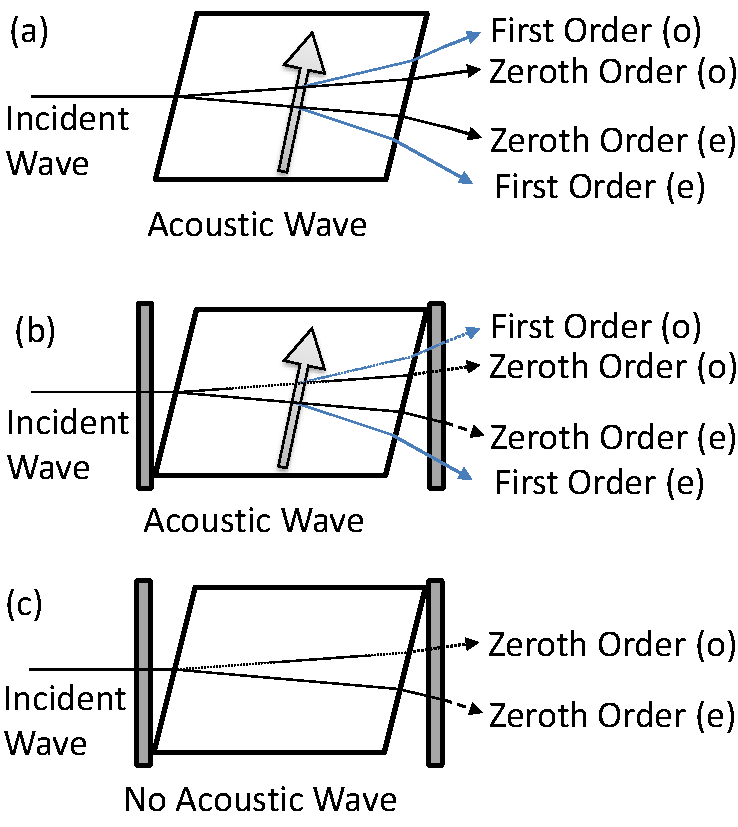
\includegraphics[height=90mm]{amt-2015-329-discussions-f02.pdf}
\caption{\textbf{(a)} A representative AOTF undergoing Bragg diffraction with an
  unpolarised incident wave with a~RF wave applied represented by the
  arrow. After the diffraction event four output signals are formed:
  the zeroth order and first order ordinary (o) and extraordinary (e)
  signals. However the only optical path that remains at a~constant
  angle no matter the applied RF wavelength is the first order
  extraordinary diffracted signal. \textbf{(b)} Two linear polarizers
  are added to the system, the first linear polarizer removes the
  ordinary polarization removing the outputs with the dotted lines and
  the second linear polarizer removes undiffracted extraordinary light
  shown by the dashed line. \textbf{(c)} The system in \textbf{(b)}
  without a~RF wave so Bragg diffraction is occurring. Once again the
  first linear polarizer removes the ordinary polarization represented
  by the dotted line and the second linear polarizer removes the
  extraordinary light shown by the dashed line.}
\label{amtd-2015-0329-f02.pdf}
\end{figure}


\end{document}

